\documentclass[conference]{IEEEtran}
\IEEEoverridecommandlockouts

\usepackage{cite}
\usepackage{amsmath,amssymb,amsfonts}
\usepackage{graphicx}
\usepackage{textcomp}
\usepackage{xcolor}
\usepackage{booktabs}
\usepackage{url}

\begin{document}

\title{A Data-Driven Analysis of Football Players' Transfer Value Based on Performance and Contract Characteristics}

\author{
\IEEEauthorblockN{David Aslanyan}
\IEEEauthorblockA{\textit{American University of Armenia}\\
Yerevan, Armenia\\
david\_aslanyan@edu.auau.am}
\and
\IEEEauthorblockN{Supervisor: Arman Asryan}
\IEEEauthorblockA{\textit{American University of Armenia}\\
Yerevan, Armenia}
}

\maketitle

\begin{abstract}
Football player market value is an important signal for recruitment, squad planning, and contract negotiation, but it is influenced by performance, age, league context, contract status, and market perception rather than one observable factor. This project builds a reproducible player-season analytics workflow for estimating Transfermarkt market value from public top-five-European-league data. The final modeling dataset contains 5,271 player-season/team observations after excluding rows with fewer than 300 minutes and stale market-value targets. Models are trained on the 2021/22 and 2022/23 seasons and evaluated on the held-out 2023/24 season. The best global model is histogram gradient boosting, with test RMSE log 0.759, MAE log 0.598, and \(R^2\) 0.622. Age, league, contract years remaining, minutes, goals per 90, and other context/performance variables emerge as important valuation signals. Segment-specific league and position models provide diagnostic insight but do not outperform the global model on matched test subsets. The main contribution is a transparent, one-command reproducible pipeline connecting data preprocessing, validation, modeling, visualization, robustness checks, and IEEE-ready reporting.
\end{abstract}

\begin{IEEEkeywords}
football analytics, market value prediction, Transfermarkt, machine learning, regression, contract analysis, reproducibility
\end{IEEEkeywords}

\section{Introduction}
Transfer values play a central role in professional football. Clubs use them in recruitment, contract negotiation, squad planning, and financial reporting, while fans and media treat them as compact summaries of player quality and potential. However, valuation is not determined only by goals or assists. It reflects a combination of age, playing time, role, league exposure, contract status, transfer history, and less observable factors such as reputation, injuries, wage demands, agent strategy, and club-specific bargaining power.

This project studies whether public season-level football data can explain a meaningful portion of player market value and which factors are most strongly associated with that value. The applied problem is important because a transparent valuation model can help identify which signals are consistently related to market perception and where public data remains insufficient. A model of this kind is not a replacement for scouting or financial negotiation, but it can provide a reproducible baseline for evaluating how observed performance, age, league, and contract information relate to the market's view of a player.

The work focuses on top-five-European-league player-season observations across 2021/22, 2022/23, and 2023/24. The modeling target is Transfermarkt market value. Transfermarkt values are useful because they provide broad public coverage, but they should be understood as a proxy for perceived market value rather than realized transfer fees. This distinction matters throughout the project: the goal is to estimate a market-perception target from public data, not to prove the exact causal price that a club would pay in a negotiation.

The research questions are:
\begin{enumerate}
    \item How accurately can football player market value be predicted from public performance, contract, transfer-history, and context features?
    \item Which features are most associated with predicted market value?
    \item Do position-specific or league-specific models improve over a single global model?
    \item How should contract-related features be interpreted when the available contract information is approximate?
\end{enumerate}

The project meets these questions through a reproducible data science workflow. It builds an analytics table, validates target and contract construction, trains baseline and nonlinear models, evaluates them on a future-season holdout, and generates the figures and tables used in this paper from code.

\section{Literature Review}
Transfermarkt values have been widely used as a proxy for football player market valuation. Herm et al. analyze the accuracy and evaluation attributes of crowd-generated Transfermarkt values, showing that the platform reflects structured market perception rather than arbitrary opinion \cite{herm2014crowd}. This makes Transfermarkt useful for applied modeling, but also means that the target is a proxy for perceived market value rather than realized transfer fees.

Muller et al. propose data-driven approaches for estimating player market value beyond crowd judgment, emphasizing that performance, popularity, and contextual signals can be combined in predictive models \cite{muller2017beyond}. Their work motivates the present project's use of both performance and non-performance features. Aydemir et al. apply ensemble learning methods to transfer value prediction and show that nonlinear methods can improve accuracy when many interacting variables are available \cite{aydemir2022ensemble}. Tamim et al. similarly frame European football valuation as a machine-learning regression problem and compare model families using contemporary player data \cite{tamim2025football}.

Contract duration is also a known valuation factor. Poli et al. discuss econometric approaches to transfer fees and player values, including the role of contract length and market conditions \cite{poli2022contract}. A longer remaining contract can increase a selling club's bargaining position, while an expiring contract may reduce the expected fee. In this project, contract variables are reconstructed from Transfermarkt transfer-history events, so they are treated as descriptive signals rather than exact legal contract records.

Prior work supports the broad hypothesis that market value is predictable from observable signals, but common limitations remain. Public datasets often miss wages, injuries, team strength, exact contract clauses, academy status, agent influence, and club demand. Many modeling exercises also rely on random splits that may overstate performance when temporally adjacent rows leak information across train and test sets. This project therefore emphasizes reproducibility, chronological validation, diagnostic analysis, and careful language about association rather than causal effect.

\section{Methodology}
\subsection{Data Sources and Row Grain}
The project combines a public top-five-European-league performance table with Transfermarkt-derived market value and transfer-history data. The base table contains player-season/team rows, allowing players who changed clubs during a season to appear separately for each team context. The final analytics table is \texttt{data/processed/player\_season\_analytics.csv}.

This row grain is useful because a player's minutes, competition, squad, and role may differ across teams even within the same season. Keeping separate player-season/team rows avoids hiding these changes through premature aggregation. It also makes the modeling task closer to how clubs inspect player performance in a particular league and team context.

The raw performance source contains standard season-level football statistics such as minutes, starts, goals, assists, shots, shots on target, crosses, interceptions, tackles won, fouls, and fouls drawn. These variables are converted into both volume and per-90-minute features. Volume fields such as minutes and starts capture availability and coach trust, while per-90 fields help compare players with different playing time.

Transfermarkt player identifiers are used as the main join key. The preprocessing step assigns IDs, excludes ambiguous exact-name matches that map to multiple Transfermarkt players, and writes unmatched or ambiguous rows to review files. This improves the reliability of later joins, because incorrect player identity would directly corrupt both the target value and the contract features.

The target is \(\log(1 + \text{market value in EUR})\), stored as \texttt{log\_market\_value\_eur}. The log transform is used because raw market values are highly right-skewed: a small number of elite players have values far above the median player.

Each season is assigned a valuation date near the end of the football season: 2022-06-30 for 2021/22, 2023-06-30 for 2022/23, and 2024-06-30 for 2023/24. For each player-season/team row, the workflow selects the nearest market-value observation around the valuation date, preferring observations in the season-end window. Observations more than 120 days from the valuation date are flagged as stale and excluded from modeling. The workflow preserves audit columns such as market-value date and days from valuation so the target-selection rule remains inspectable.

\subsection{Preprocessing and Validation}
The preprocessing workflow assigns Transfermarkt player IDs, builds season valuation dates, selects market-value targets, parses transfer-history events, derives contract features, and joins all features into the final analytics table. Exact-name Transfermarkt matches that map to multiple player IDs are excluded and written to review files. Market-value observations more than 120 days away from the season valuation date are flagged as stale and excluded from modeling.

Contract features are derived from the latest known transfer event at or before the valuation date. This avoids future transfer leakage. If the inferred contract expiry is before the valuation date, the model uses a separate \texttt{contract\_expired} flag and caps modeled \texttt{contract\_years\_remaining} at zero. The reproduction workflow validates non-empty Transfermarkt IDs, duplicate row grains, stale targets, future-dated transfer leakage, and negative modeled contract years before modeling.

The raw transfer-history data is event-level rather than a clean season-by-season contract table, so it must be transformed carefully. The workflow parses transfer events, keeps transfer dates, transfer type, contract-until dates, market value at transfer, fees where available, and transfer counts before the valuation date. Missing contract dates are represented with an explicit \texttt{contract\_missing} indicator rather than silently dropping rows. Additional transfer-history features include days since last transfer, transfer count before valuation, and loan count before valuation.

These contract features are approximate. They are useful because they encode public information about bargaining position and player movement history, but they are not official legal contract records. The paper therefore interprets contract years remaining as a predictive signal, not as a causal estimate of the value added by one more contract year.

The project also writes intermediate datasets to make the pipeline auditable. Important outputs include ID-enriched metrics, valuation-date metrics, transfer-history events, player-season market values, player-season contract features, the final analytics table, and the final modeling dataset. This structure makes it possible to inspect each transformation stage rather than treating the model input as a black box.

\subsection{Feature Set}
The model uses age, squared age, minutes, starts, 90s, per-90 performance rates, league, season, position group, contract years remaining, expired/missing contract indicators, days since last transfer, and transfer/loan counts. The final modeling filter keeps players with at least 300 minutes, balancing coverage with removal of very small playing-time samples. A stricter 900-minute threshold is tested as a sensitivity scenario.

The resulting modeling dataset contains 5,271 rows: 3,548 training rows from 2021/22 and 2022/23, and 1,723 test rows from 2023/24. The position split is 1,488 defenders, 2,279 midfielders, and 1,504 forwards. Goalkeepers are excluded from the main modeling comparison because their performance profile differs substantially from outfield players and the available feature set is mostly outfield-oriented.

\subsection{Models and Evaluation}
Four global model families are compared: a mean baseline, ordinary least squares regression, ridge regression, and histogram gradient boosting. The mean baseline establishes a minimum reference point. Linear regression and ridge regression provide interpretable baselines and help identify whether the signal is mostly additive. Histogram gradient boosting can model nonlinear interactions among age, league, role, minutes, and contract context. Position-specific and league-specific models are also trained and compared with the corresponding global-model predictions on the same subgroup.

This segmented comparison tests whether smaller specialized estimators outperform a global model or whether the global model benefits from the larger training sample while still using league and position as features. This is important because specialized football models can sound intuitively attractive, but the empirical question is whether the loss of training data is offset by a more homogeneous subgroup.

Performance is measured with RMSE, MAE, and \(R^2\) on the log target. Euro-scale MAE is also reported after inverse transformation, but it is more sensitive to high-value outliers. Robustness checks include sensitivity experiments, bootstrap intervals for the best global model, and rolling season validation.

\section{Results}
\subsection{Global Model Performance}
Table~\ref{tab:global-metrics} shows the global test results on the held-out 2023/24 season. Histogram gradient boosting is the best global model, reducing RMSE log from 1.238 for the mean baseline to 0.759. This is a 38.7\% improvement over the baseline. Linear regression and ridge also perform strongly, with RMSE log around 0.790, confirming that public football and context variables contain substantial valuation signal.

\begin{table}[htbp]
\caption{Global model performance on the 2023/24 test season}
\label{tab:global-metrics}
\centering
\resizebox{\linewidth}{!}{
\begin{tabular}{lrrrr}
\toprule
Model & RMSE & MAE & \(R^2\) & MAE EUR \\
\midrule
Mean baseline & 1.238 & 1.024 & -0.005 & 10.99M \\
Linear regression & 0.790 & 0.631 & 0.591 & 7.48M \\
Ridge & 0.790 & 0.631 & 0.591 & 7.47M \\
Hist. gradient boosting & \textbf{0.759} & \textbf{0.598} & \textbf{0.622} & \textbf{6.86M} \\
\bottomrule
\end{tabular}}
\end{table}

\begin{figure}[htbp]
\centerline{
\includegraphics[width=\linewidth]{figures/model_comparison_test_rmse.png}}
\caption{Global model comparison on the 2023/24 test season.}
\label{fig:model-comparison}
\end{figure}

Figure~\ref{fig:model-comparison} visualizes the global RMSE comparison. The nonlinear model's advantage suggests that valuation is not purely additive or linear. For example, the same goal rate may be interpreted differently depending on age, position, league, and playing-time volume. The linear models still perform well, which indicates that some market-value structure is captured by broad, stable signals such as age, minutes, league, and position.

\subsection{Prediction Calibration and Residuals}
Figure~\ref{fig:predicted-actual} compares predicted and actual log market values for the best model. The model captures the general ordering of players, but errors remain for outliers. This is expected because public performance and contract features do not fully observe reputation, injury history, wage level, club need, or transfer-market demand.

\begin{figure}[htbp]
\centerline{
\includegraphics[width=\linewidth]{figures/predicted_vs_actual_best_model.png}}
\caption{Predicted versus actual log market value for the best global model.}
\label{fig:predicted-actual}
\end{figure}

Error diagnostics show that the Premier League has the lowest MAE log among league groups, while Bundesliga has the highest MAE log in the best global model's test predictions. By position, forwards have the lowest RMSE log, followed by midfielders and defenders. These differences should be interpreted as reliability diagnostics rather than evidence that one group is inherently easier to value in all settings.

\begin{figure}[htbp]
\centerline{
\includegraphics[width=\linewidth]{figures/residuals_by_league_position.png}}
\caption{Residuals by league and position for the best global model.}
\label{fig:residuals}
\end{figure}

\subsection{Feature Importance}
Permutation importance for the best nonlinear model highlights age, league, contract years remaining, 90s, goals per 90, minutes, assists per 90, shots per 90, days since last transfer, and crosses per 90. Ridge coefficients provide a complementary linear view: age and age squared are large in opposite directions, consistent with a nonlinear age-value pattern where younger players carry resale potential but value does not increase indefinitely with youth alone.

\begin{table}[htbp]
\caption{Top permutation-importance features for the best global model}
\label{tab:importance}
\centering
\begin{tabular}{lr}
\toprule
Feature & RMSE increase \\
\midrule
Age & 0.285 \\
League & 0.161 \\
Contract years remaining & 0.074 \\
90s & 0.053 \\
Goals per 90 & 0.046 \\
Minutes & 0.042 \\
Assists per 90 & 0.036 \\
Shots per 90 & 0.032 \\
Days since last transfer & 0.028 \\
Crosses per 90 & 0.024 \\
\bottomrule
\end{tabular}
\end{table}

These results align with football intuition: age captures future potential and depreciation; league captures market context; contract duration captures bargaining position; minutes and starts capture trust and availability; attacking output captures visible contribution. The findings are associational and should not be read as causal estimates. For example, high minutes may indicate quality, but they may also reflect squad depth, manager preference, or injury luck. Similarly, a longer contract can increase market value through bargaining position, but it may also be correlated with clubs choosing to secure already valuable players.

\subsection{Segment-Specific Models}
Position-specific and league-specific models were trained to test whether smaller specialized estimators outperform a global model. Figure~\ref{fig:specialized-global} shows that the global histogram gradient boosting model performs better than specialized histogram gradient boosting in every tested segment. The likely explanation is sample size: the global model can learn shared valuation structure across leagues and positions while still using league and position as features.

\begin{figure}[htbp]
\centerline{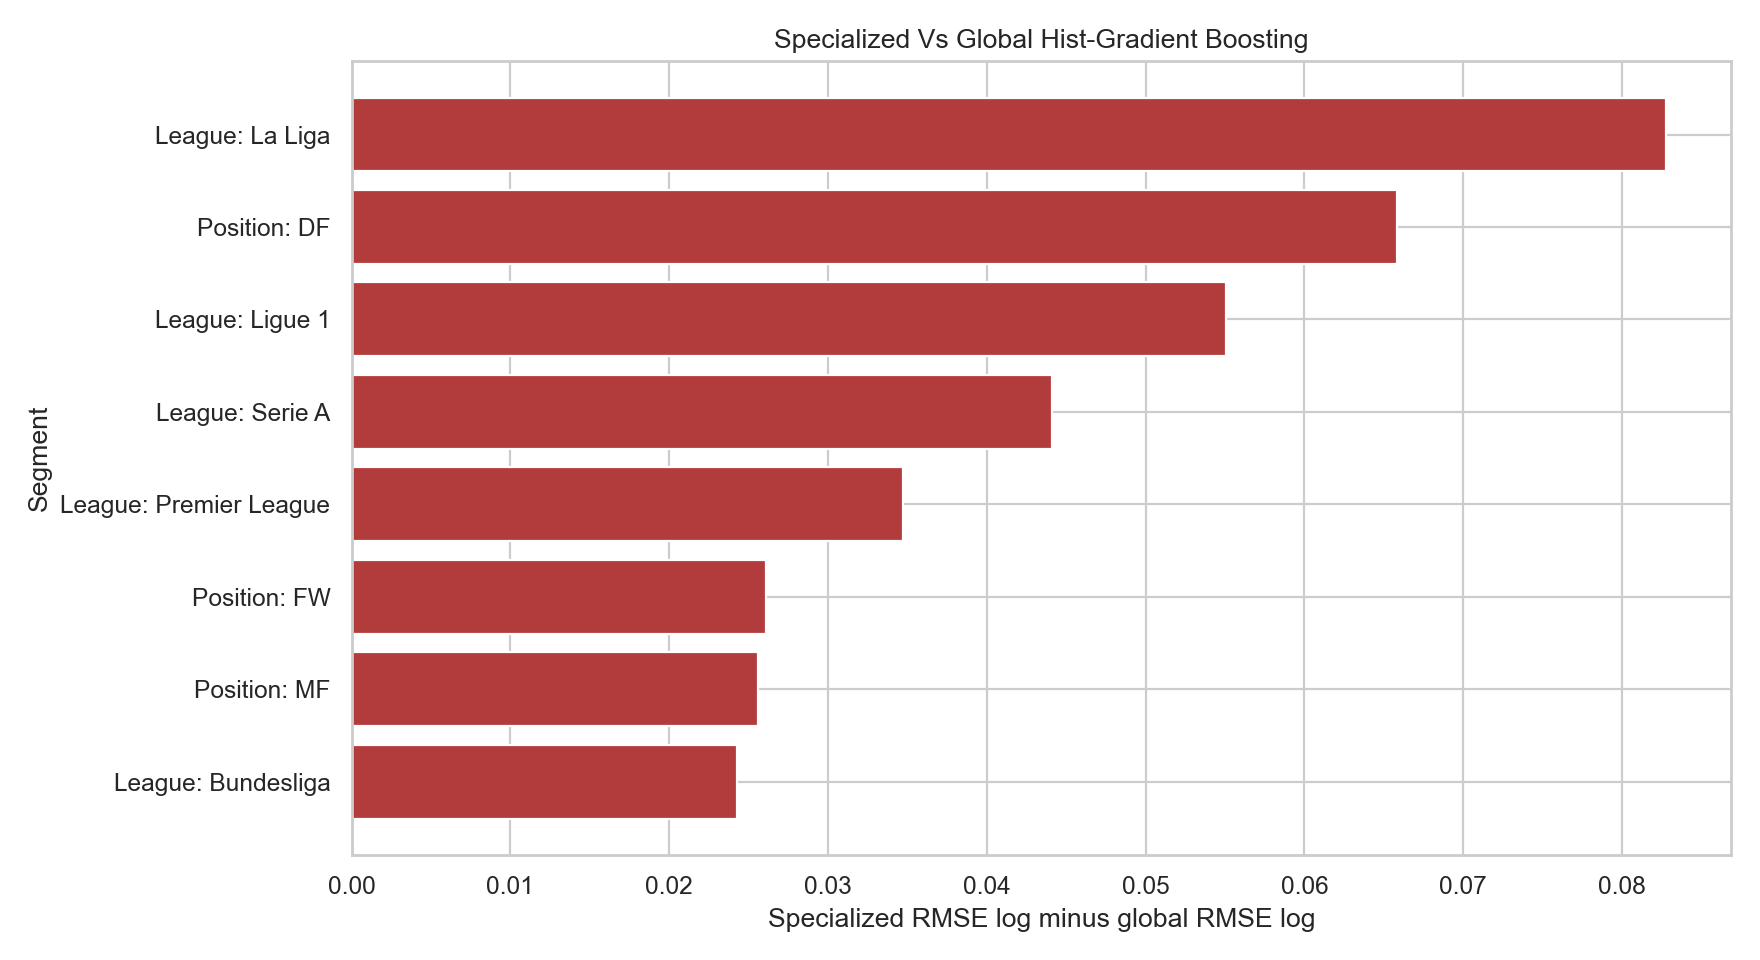
\includegraphics[width=\linewidth]{figures/specialized_vs_global_rmse.png}}
\caption{Segment-specific histogram gradient boosting models compared with the global model on the same subgroup. Positive values favor the global model.}
\label{fig:specialized-global}
\end{figure}

Specialized models remain useful diagnostically. For example, they show that league and position groups differ in error profile and may have distinct valuation mechanisms. However, they are not the best headline prediction strategy for this dataset. This is an important negative result because it prevents a tempting but unsupported conclusion that separate models are always better for each football role or league.

\begin{figure}[htbp]
\centerline{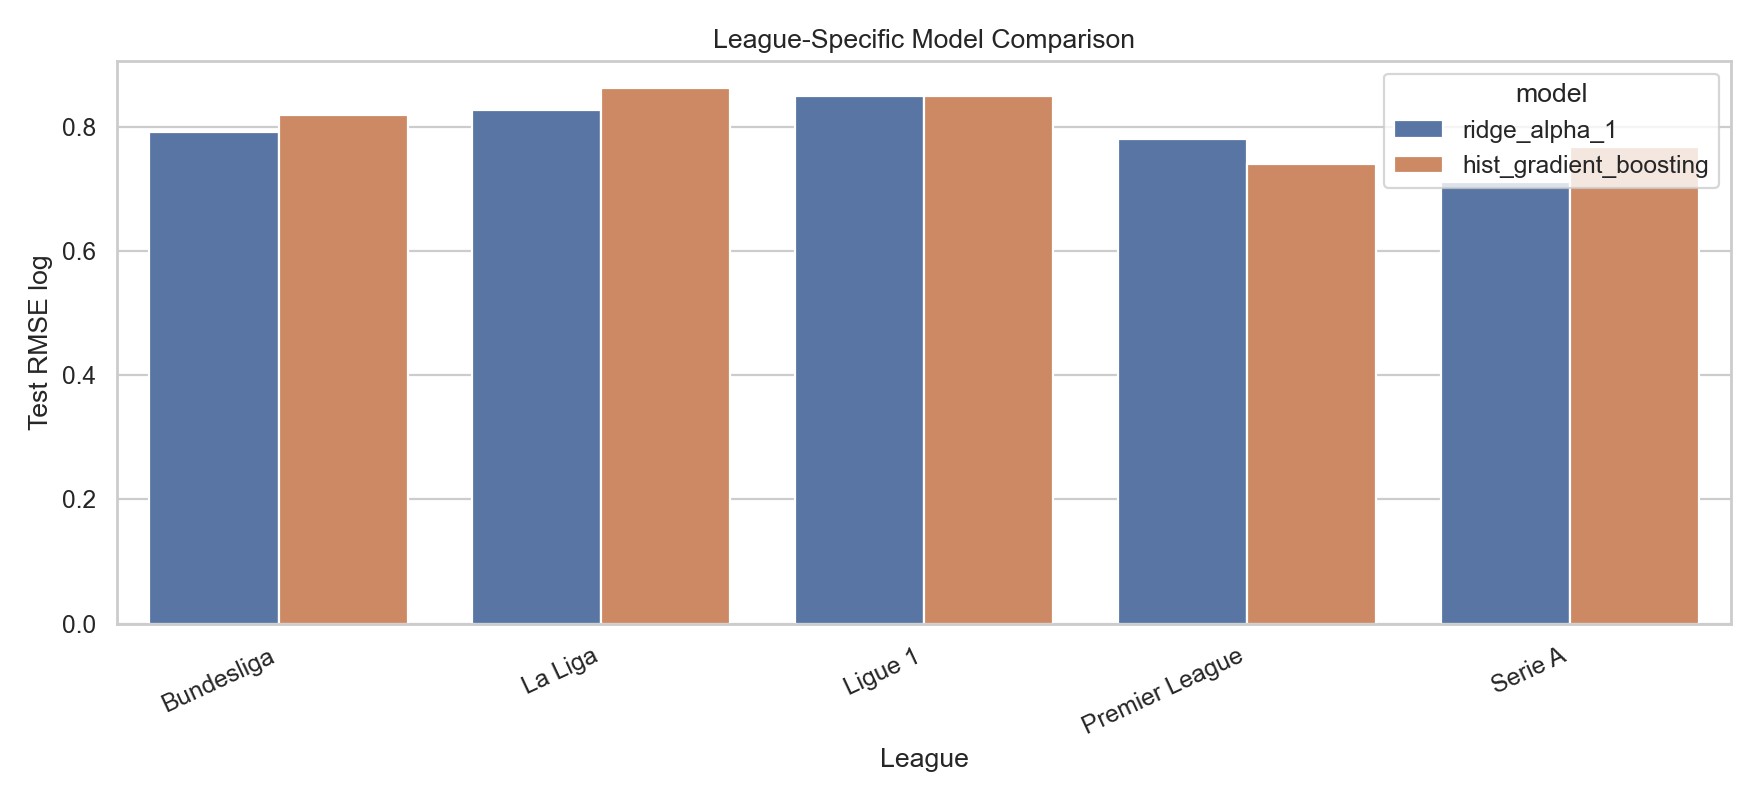
\includegraphics[width=\linewidth]{figures/league_model_comparison.png}}
\caption{League-specific model comparison on the held-out test season.}
\label{fig:league-models}
\end{figure}

\begin{figure}[htbp]
\centerline{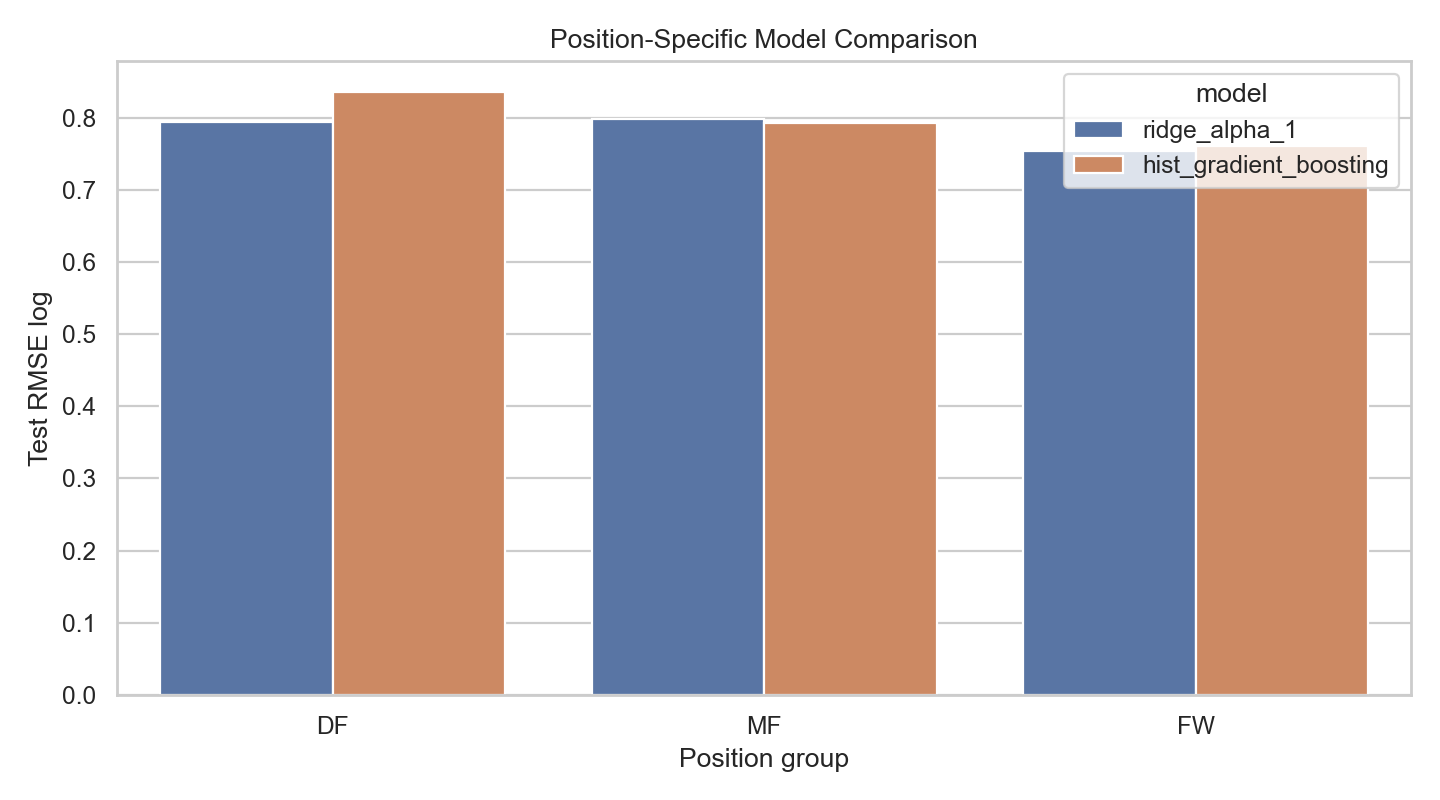
\includegraphics[width=\linewidth]{figures/position_model_comparison.png}}
\caption{Position-specific model comparison on the held-out test season.}
\label{fig:position-models}
\end{figure}

\section{Analysis and Validation}
\subsection{Robustness Checks}
Table~\ref{tab:sensitivity} summarizes the main sensitivity scenarios. Removing contract and transfer-history features worsens histogram gradient boosting RMSE log from 0.759 to 0.815, indicating that contract and transfer-history variables add meaningful predictive signal. Restricting to in-window target values produces nearly identical performance, which supports the target-selection rule. A stricter 900-minute threshold improves RMSE log to 0.735 but reduces the test set from 1,723 to 1,303 rows, reflecting a tradeoff between cleaner regular-starter samples and broader player coverage.

\begin{table}[htbp]
\caption{Sensitivity checks for histogram gradient boosting}
\label{tab:sensitivity}
\centering
\resizebox{\linewidth}{!}{
\begin{tabular}{lrrr}
\toprule
Scenario & Rows & RMSE & \(R^2\) \\
\midrule
All features, 300 min & 1723 & 0.759 & 0.622 \\
No contract/transfer & 1723 & 0.815 & 0.564 \\
In-window targets only & 1722 & 0.761 & 0.620 \\
All features, 900 min & 1303 & 0.735 & 0.620 \\
\bottomrule
\end{tabular}}
\end{table}

Bootstrap resampling of 2023/24 test residuals gives a 95\% interval of 0.732 to 0.787 for RMSE log and 0.577 to 0.620 for MAE log. Rolling season validation is also consistent: testing 2022/23 after training on 2021/22 gives histogram gradient boosting RMSE log 0.759 and \(R^2\) 0.611, close to the final 2023/24 holdout performance.

\begin{table}[htbp]
\caption{Rolling Season Validation for Histogram Gradient Boosting}
\label{tab:rolling}
\centering
\resizebox{\linewidth}{!}{
\begin{tabular}{llrrr}
\toprule
Train & Test & Rows & RMSE & \(R^2\) \\
\midrule
21/22 & 22/23 & 1764 & 0.759 & 0.611 \\
21/22, 22/23 & 23/24 & 1723 & 0.759 & 0.622 \\
\bottomrule
\end{tabular}}
\end{table}

\subsection{Objective Assessment}
The project meets its primary predictive objective: all learned global models outperform the mean baseline on a future-season holdout. It also meets the interpretability objective by identifying stable feature groups associated with valuation. The segmentation objective is met with a negative result: specialized models are informative, but the global model is more reliable as the headline estimator. The contract objective is partially met: contract years remaining is predictive, but the feature is reconstructed from transfer-history events and must be interpreted cautiously.

The validation design is stronger than a random row split because it asks whether models trained on earlier seasons generalize to a later season. This is closer to a real deployment setting, where a model would be trained on past observations and used to evaluate current or future players. The rolling validation check further supports the conclusion that the result is not tied to one arbitrary train/test year.

\subsection{Limitations}
Several limitations remain. Transfermarkt values are estimates of market perception rather than confirmed transfer fees. Contract expiry data is approximate and event-derived rather than a complete official contract database. The dataset does not include wages, injuries, team strength, tactical role, European competition participation, academy status, agent influence, or actual club demand. The data also covers only three seasons, limiting the depth of temporal validation. These limitations explain why the model has moderate rather than near-perfect accuracy.

Another limitation is feature coverage across positions. Outfield event types such as goals, assists, shots, crosses, interceptions, and tackles are useful, but they do not fully describe defensive positioning, pressing, ball progression, chance creation, or goalkeeper performance. This is why the current paper treats the model as a transparent public-data baseline, not as a complete professional recruitment system.

\section{Discussion and Conclusion}
This project demonstrates that football player market value can be estimated with meaningful accuracy from public season-level performance, contract, transfer-history, and context data. The best model explains a substantial share of variance on a future-season holdout, with RMSE log 0.759 and \(R^2\) 0.622. The strongest signals are age, league, contract years remaining, playing-time volume, and attacking-output variables.

The main contribution is not only the model result, but the reproducible workflow. A single command regenerates the ID-enriched data, analytics table, validation checks, modeling dataset, figures, tables, Markdown report, and paper-ready figure assets. This directly supports the capstone requirement that figures and tables be reproducible from code.

Future work should add richer event-level performance features such as expected goals, expected assists, progressive passes, carries, pressures, blocks, aerials, and goalkeeper-specific metrics. It should also add club strength, wages, injury history, official contract data, and external validation against realized transfer fees. With these additions, the model could move from a transparent academic valuation analysis toward a more complete recruitment-support tool.

\section*{Acknowledgment}
The student thanks Arman Asryan and the American University of Armenia for guidance and support.

\bibliographystyle{IEEEtran}
\bibliography{references}

\end{document}
